\documentclass[a4paper,12pt]{article}
\usepackage[utf8]{inputenc}
\usepackage{amsmath, amssymb, amsthm}
\usepackage{geometry}
\geometry{a4paper, margin=20mm, top=25mm, bottom=25mm}
\usepackage{multicol}
\usepackage{enumitem}
\usepackage[T1]{fontenc}
\usepackage[serbian]{babel} % Podeseno za latinicu
\usepackage{mathtools,amsfonts}
\usepackage{hyperref}
\usepackage{titlesec}
\usepackage{algorithm}
\usepackage{algpseudocode}
\makeatletter
\renewcommand{\ALG@name}{Algoritam}
\numberwithin{algorithm}{section}
\makeatother

\hypersetup{
    colorlinks=true,
    citecolor=black,
    filecolor=black,
    linkcolor=black,
    urlcolor=blue
}

% Podesavanje naslova sekcija
\titleformat{\section}{\normalfont\large\bfseries}{\thesection.}{0.5em}{}
\titleformat{\subsection}{\normalfont\normalsize\bfseries\itshape}{\thesubsection.}{0.5em}{}

% Matematicke okoline na latinici
\theoremstyle{plain}
\newtheorem{theorem}{Teorema}[section]
\newtheorem{lemma}[theorem]{Lema}
\newtheorem{corollary}[theorem]{Posledica}

\theoremstyle{definition}
\newtheorem{definition}{Definicija}[section]
\newtheorem{example}{Primer}[section]

\theoremstyle{remark}
\newtheorem*{remark}{Napomena}

% Definicija lokalnih matematickih funkcija standardnih za nase podrucje
\renewcommand{\tan}{\operatorname{tg}}
\newcommand{\coloneqq}{\mathrel{\mathop:}=}
\renewcommand{\cot}{\operatorname{ctg}}
\renewcommand{\arctan}{\operatorname{arctg}}
\newcommand{\arccot}{\operatorname{arcctg}}

\begin{document}

% Glavni naslov u stilu sa slike
\begin{center}
    \vspace*{5mm}
    {\large\bfseries Ispitna pitanja iz Diskretnih struktura 2 (Informatika)} \\
    \vspace{2mm}
    {\large\bfseries --- Odgovori na pitanja ---} \\
    \vspace{2mm}
    {\large\bfseries 2025/2026} \\
    \vspace{4mm}
    {\itshape Kosta Čolović} \\
    \vspace{2mm}
    {\small Poslednja izmena: \today}
\end{center}
\vspace{8mm}
\textit{Na kraju dokumenta se nalazi sadržaj, radi brže navigacije.}


\section{Prebrojavanja. Osnovni principi prebrojavanja. (Uopšteni) Dirihleov princip.}
Prebrojati skup znači odrediti njegovu kardinalnost.\\

\noindent Osnovni principi prebrojavanja:
\begin{enumerate}
    \item \textbf{Princip jednakosti}: Ukoliko za skupove $A$ i $B$ postoji bijekcija $f: A \to B$, tada važi \[|A| = |B|\]
    \item \textbf{Princip zbira}: Ako su konačni skupovi $A_1, A_2, \ldots, A_n$ disjunktni, tada važi \[\bigg|\bigcup_{i = 0}^n A_i \bigg| = \sum_{i = 0}^{n} | A_i |\]
    \item \textbf{Princip proizvoda}: Ako su $A$ i $B$ proizvoljni konačni skupovi, tada važi
    \[ |A \times B| = |A| \cdot |B| \]
    Važi i opštije tvrđenje. Neka je \[S \subseteq A \times B,\;\; v_a = \{(a, b) \in S \;|\; b \in B\}\; \text{i} \; k_a = \{(a, b) \in S \;|\; a \in A\}.\]
    Tada važi 
    \[ |S| = \sum_{a \in A} |v_a| = \sum_{b \in B} |k_b|\]
\end{enumerate}

\begin{itemize}
    \item \textbf{Dirihleov princip}: Ako je $k$ objekata raspoređeno u $n < k$ kutija, tada u bar jednoj kutiji ima bar 2 objekta.
    \item \textbf{Uopšteni Dirihleov princip}: Ako je $k$ objekata raspoređeno u $n$ kutija i $k > cn$, tada u bar jednoj kutiji ima bar $c + 1$ objekat.
\end{itemize}
\subsection{Ramzijevi brojevi}
\begin{itemize}
    \item \textbf{Ramzijev broj} $R(n, k)$ označava najmanji skup osoba takav da u njemu postoji ili $k$ osoba koje se poznaju ili $n$ osoba koje se ne poznaju. Zapravo, $R(n, k)$ predstavlja najmanji broj $m$ td. svako bojenje grafa $K_m$ sa dve boje sadrži potpun monohromatski podgraf sa $n$ ili $k$ čvorova. Samo nekoliko vrednosti je poznato, jer je algoritam eksponencijalne složenosti. Npr, $R(3, 3) = 6$.
\end{itemize}

\section{Binomni koeficijenti. Osnovna svojstva. Binomna i polinomna formula. }

\[
    {{n}\choose k} = \frac{n(n-1)(n-2)\dots(n-k+1)}{k!}, \;\; k \in \mathbb{N}, \; n \in \mathbb{R}, \;\; {{n}\choose 0} = 1
\]\\

Za $k \leq n$ važi
\[
    {{n}\choose k} = \frac{n!}{(n-k)!k!}
\]

\begin{theorem} \textbf{(Uslov simetričnost):}
    Za $k, n \in \mathbb{N}, k \leq n$ važi
    \[
        {{n} \choose k} = {{n} \choose {n-k}}
    \]
\end{theorem}
\begin{proof}
    \[
        {{n} \choose k} = \frac{n!}{k!(n - k)!} = \frac{n!}{(n-k)! (n - (n-k))!} = {{n} \choose {n-k}}
    \]
\end{proof}

\begin{theorem}
    \textbf{(Negacija gornjeg indeksa:)}
     Za $k \in \mathbb{N}, n \in \mathbb{R}$ važi
     \[ {{-n} \choose k} = (-1)^k {{n + k - 1} \choose k} \]
\end{theorem}
\begin{proof}
    \[
        {{-n} \choose k} = \frac{(-n)(-n - 1)\ldots (-n - k + 1)}{k!} = 
    \]
    \[
        =(-1)^k \frac{n(n-1)\ldots(n + k - 1)}{k!} = (-1)^k {{n + k - 1} \choose k}
    \]
\end{proof}

\begin{theorem}
    \textbf{(Adiciona formula):} Za $k \in \mathbb{N}$ i $n \in \mathbb{R}$ važi
    \[ {{n} \choose k} = {{n - 1} \choose k} + {{n - 1} \choose {k - 1}} \]
\end{theorem}
\begin{proof}
    \[
        {{n - 1} \choose k} + {{n - 1} \choose {k - 1}} = \frac{(n - 1)\ldots (n - k)}{k!} + \frac{(n - 1)\ldots (n - k + 1)}{(k - 1)!}
    \]
    \[
        = \frac{(n - 1)\ldots (n - k) + k(n - 1)\ldots (n - k + 1)}{k!} = \frac{(n - 1)\ldots(n - k + 1)(n - k + k)}{k!} = {{n} \choose k}
    \]
\end{proof}

\subsection{Binomna i polinomna formula}
\begin{theorem}
    \textbf{(Binomna formula):} Za $n \in \mathbb{N}_0,\; x,y \in \mathbb{R}$ važi
    \[
        (x + y)^n = \sum_{k = 0}^{n} {{n} \choose k}x^k y^{n - k}
    \]
\end{theorem}
\begin{proof}
    Indukcija po $n$. Za $n = 0$ je $1 = (x+y)^n = 1$. Pretpostavimo da formula važi za $n - 1$. Tada dobijamo
    \[
        \begin{aligned}
            (x + y)^n &= (x+y) \sum_{k = 0}^{n - 1}{{n - 1} \choose k}x^k y^{n - 1 - k}\\
            &= \sum_{k = 0}^{n-1}{{n - 1} \choose k}x^{k + 1}y^{n - 1 - k} + \sum_{k = 0}^{n - 1} {{n - 1} \choose k}x^k y^{n - k} \\
            &= x^n + \sum_{k = 1}^{n-1}{{n - 1} \choose {k-1}}x^{k + 1}y^{n - 1 - k} + y^n + \sum_{k = 1}^{n - 1} {{n - 1} \choose k}x^k y^{n - k} \\
            &= x^n + y^n + \sum_{k = 1}^{n - 1}\bigg({{n - 1} \choose k-1} + {{n - 1} \choose {k}} \bigg) x^k y ^{n-k} \\
            &= x^n + y^n + \sum_{k = 1}^{n - 1}{{n} \choose k}x^k y^{n - k}\\ 
            &= {{n} \choose n} x^n + {{n} \choose 0} y^n + \sum_{k = 1}^{n - 1}{{n} \choose k}x^k y^{n - k} \\
            &= \sum_{k = 0}^{n}{{n} \choose k}x^k y^{n - k}
        \end{aligned}
    \]
\end{proof}

\begin{theorem}
    \textbf{(Polinomna formula):} Za $n \in \mathbb{N}_0$ i $x_1, \ldots, x_r \in \mathbb{R}$ važi
    \[ \bigg(\sum_{k = 1}^{r}x_k\bigg)^n = \sum_{\substack{k_1 + k_2 + \dots + k_r = n \\ k_1, k_2, \dots, k_r \geq 0}} {{n}\choose k_1, k_2, \dots, k_r} x_1^{k_1} x_2^{k_2} \dots x_r^{k_r},\]
   gde je \[ {{n}\choose k_1, k_2, \dots, k_m} = \frac{n!}{k_1! k_2! \dots k_m!}. \]
\end{theorem}
\begin{proof}
    Dokaz se može izvesti indukcijom po $r$.
\end{proof}
\newpage
\section{Binomni identiteti.}

\begin{theorem}
    \textbf{(Izvlačenje ispred zagrade):} Za $k, n \in \mathbb{N}$ važi:
    \[ {{n} \choose k} = \frac{n}{k} {{n - 1} \choose {k - 1}}, \; {{n} \choose {k}} = \frac{n}{n-k} {{n - 1} \choose k} \]
\end{theorem}
\begin{proof}
    Za $k > n$ oba identiteta slede direktno.
\end{proof}

\begin{theorem}
    \textbf{(Pojednostavljivanje proizvoda):} Za $k, n, r \in \mathbb{N}_0$ važi
    \[ {{n} \choose k + r}{{k + r} \choose k} = {{n} \choose k}{{n - k} \choose r} \]
\end{theorem}
\begin{proof}
    Dobija se direktno.
\end{proof}

\begin{theorem}
    \textbf{(Sumacione formule):} Za $r, n \in \mathbb{N}_0$ važi
    \[ \sum_{k= 0}^{n}{{r + k} \choose k} = {{n + r + 1}\choose n}, \;\;\;   \sum_{k= 0}^{n}{{k} \choose r} = {{n + 1}\choose r + 1}\]
\end{theorem}
\begin{proof}
    Identiteti se dokazuju indukcijom.\\
    Dokažimo prvo prvi identitet. Za $n = 0$ imamo $1 = 1$. Pretpostavimo da važi za $n - 1$.
    \[ \sum_{k = 0}^{n} {{r + k} \choose k} = \sum_{k = 0}^{n - 1}{{r + k} \choose k} + {{r + n} \choose n} = {{r + n} \choose {n - 1}} + {{r + n} \choose n} = {{n + r + 1} \choose n} \] \\

    \noindent Dokažimo sada drugi identitet. Za $n = 0$ imamo $1 = 1$. Pretpostavimo da važi za $n - 1$.
    \[ \sum_{k = 0}^{n} {{k} \choose r} = \sum_{k = 0}^{n-1} {{k} \choose r} + {{n} \choose r} = {{n} \choose {r + 1}} + {{n} \choose r} = {{n + 1} \choose {r + 1}} \]
\end{proof}

\begin{theorem}
    \textbf{(Suma kvadrata):} Za $n \in \mathbb{N}_0$ važi
    \[ \sum_{k = 0}^{n} {{n} \choose k}^2 = {{2n} \choose n} \]
\end{theorem}
\begin{proof} Koeficijenti u z $x^n$ u narednim jednakostima moraju biti jednaki
    \[  \sum_{k = 0}^{2n}{{2n} \choose k} x^k = (x + 1)^{2n} = (x+1)^n (x+1)^n = \bigg(\sum_{k = 0}^{n}{{n} \choose k}x^k\bigg)\bigg(\sum_{k = 0}^{n}{{n} \choose k}x^{n-k}\bigg)  \]
    \[ \implies \sum_{k = 0}^{n} {{n} \choose k}^2 = {{2n} \choose n} \]
\end{proof}
\newpage

\section{Princip uključenja-isključenja.}

\begin{theorem}
    Za konačne skupove $A_1, A_2, \ldots, A_n$ važi
    \[ \Bigg| \bigcup_{i = 1}^n A_i \Bigg| = \sum_{\emptyset \neq I \subset \mathbb{N}_n} (-1)^{|I| - 1} \Bigg| \bigcap_{i \in I} A_i \Bigg|\]
\end{theorem}

\begin{proof}
    \[x \in \bigcup_{i = 1}^n A_i \implies x \;\text{pripada nekim od } A_1, A_2, \ldots, A_n\]
Bez umanjenja opštosti, neka $x$ pripada skupovima $A_1, A_2, \ldots, A_k$. Tada važi
\[ x \in \bigcap_{i = 1}^k A_i \]
Dakle, $x$ doprinosi da se vrednost sa leve strane teoreme uveća za 1. Treba dokazati da to važi i za desnu stranu. Naime, doprinos elementa $x$ desnoj strani jednak je
\[ k - {{k} \choose 2} + {{k} \choose 3} - \ldots + (-1)^{k-1}{{k} \choose k} = {{k} \choose 0} - \sum_{i = 0}^{k}{{k} \choose i}(-1)^i = 1 - 0 = 1 \]
\end{proof}

\section{Uređeni izbori elemenata sa i bez ponavljanja. Permutacije. }
\begin{itemize}
    \item \textbf{Uređeni} izbori elemenata (\textbf{varijacije} ili \textbf{permutacije $k$-tog reda}) su oni kod kojih bitan redosled izbora.
\end{itemize}
\subsection{Uređeni izbori sa ponavljanjem}
\begin{theorem}
    Broj preslikavanja $f: \mathbb{N}_k \rightarrow \mathbb{N}_n$ jednak je $n^k$.
\end{theorem}
\begin{proof}
    Indukcijom po $k$. Za $k = 1$ postoji $n$ preslikavanja. Pretpostavimo da tvrdnje važi za $k-1$.
    Dakle, $k - 1$ element skupa $\mathbb{N}_k$ se u $\mathbb{N}_n$ može preslikati na $n^{k - 1}$ način. Preostali element se može preslikati u bilo koji od $n$ elemenata iz $\mathbb{N}_n$. Dakle, ukupan broj je $n^{k - 1} \cdot n = n^k$.
\end{proof}
\begin{definition}
    Neka je $A$ proizvoljni podskup skupa $X$. \textbf{Karakteristična funkcija} skupa $A$, $\chi_A : X \rightarrow \{0, 1\}$, definisana je sa
    \[ \chi_A = \begin{cases}
        1,\;\; x \in A, \\
        0,\;\; x \not\in A.
    \end{cases} \]
\end{definition}

\begin{theorem}
    Neka je $X$ skup od $n$ elemenata. Tada važi
    \[ |P(X)| = 2^n \]
\end{theorem}
\begin{proof}
    Svakom podskupu skupa $X$ odgovara jedna karakteristična funkcija, a i svakoj karakterističoj funkciji odgovara jedan podskup. Ovih funkcija ima $2^n$.
\end{proof}
\newpage
\subsection{Uređeni izbori bez ponavljanja}
\begin{itemize}
    \item Broj uređenih izbora $k$ elemenata skupa od $n$ elemenata jednak je broju injektivnih preslikavanja $f: \mathbb{N}_k \rightarrow \mathbb{N}_n$.
\end{itemize}
\begin{theorem}
    Za prirodne brojeve $n$ i $k$ td. $k \leq n$, broj injektivnih preslikavanja $f: \mathbb{N}_k \rightarrow \mathbb{N}_n$ jednak je
    \[ \prod_{i = 0}^{k - 1} (n-i)  = \frac{n!}{(n-k)!}\]
\end{theorem}

\begin{proof}
    Indukcijom po $k$. Za $k = 1$, imamo $n$ preslikavanja, slično kao ranije. Pretpostavimo da tvrdnje važi za $k - 1$. Sada prvih $k - 1$ elemenata skupa $\mathbb{N}_k$ možemo na $n(n-1)\dots(n - k + 2)$ načina preslikati u skup $\mathbb{N}_n$. Kako su u pitanju izbori bez ponavljanja, preostali element možemo pridružiti jednom od $n - k + 1$ elemenata. Dakle, ukupan broj načina je 
    \[ n(n-1)\dots (n - k + 1) \]
\end{proof}

\begin{itemize}
    \item \textbf{Permutacije} su specijalan slučaj u kom važi $n = k$. Dakle, broj permutacija je $n!$.
    \item Za veliko $n$, faktorijel se može aproksimirati \textbf{Stirlingovom formulom}: \[ n! \approx \sqrt{2\pi n}\bigg(\frac{n}{e}\bigg)^n \]
\end{itemize}

\section{Neuređeni izbori elemenata sa i bez ponavljanja. Permutacije sa ponavljanjem.}
\begin{itemize}
    \item \textbf{Neuređeni} izbori elemenata (\textbf{kombinacije}) su oni kod kojih je nebitan redosled elemenata.
\end{itemize}
\subsection{Neuređeni izbori bez ponavljanja}
\begin{theorem}
    Neka su $k, n \in \mathbb{N}, \; k \leq n$. Broj Neuređenih izbora $k$ elemenata skupa od $n$ elemenata je 
    \[ {{n} \choose k} = \frac{n!}{k!(n-k)!} \]
\end{theorem}
\begin{proof}
    Kako je broj uređenih izbora $k$ od $n$ elemenata jednak $\frac{n!}{(n-k)!}$, a nama trebaju neuređeni izbori, treba podeliti ovaj količnik sa $k!$.
\end{proof}
\newpage
\begin{theorem}
    \textbf{(Vandermondov identitet):}
    \[{{r}\choose {0}}{{s} \choose n} + {{r} \choose 1}{{s} \choose {n-1}} + {{r} \choose 2}{{s} \choose n - 2} + \dots + {{r} \choose r}{{s} \choose n - r} = {{r+s} \choose n}\]
\end{theorem}
\begin{proof}
    Neka se u prostoriji nalazi $r$ devojčica i $s$ dečaka. Neka je potrebno izabrati $n$ dece nezavisno od pola. To se može uraditi na ${{r+s}\choose n}$ načina. \\

    Sa druge strane, $k$ devojčica možemo izabrati na ${{r} \choose k}$ načina, dok $n - k$ dečaka možemo odabrati na ${{s} \choose {n-k}}$. Sumiranjem po $k$ dobijamo da je ukupan broj načina za odabir $n$ dece
    \[ \sum_{k = 0}^{r}{{r} \choose k}{{s} \choose {n-k}} \]
\end{proof}

\begin{theorem}
    \[ {{r} \choose 0}{{s} \choose n} + {{r} \choose 1}{{s} \choose n + 1} + {{r} \choose 2}{{s}\choose n + 2} + \dots + {{r} \choose r}{{s} \choose {{n + r}}} = {{r + s} \choose {r + n}} \]
\end{theorem}
\begin{proof}
    Prema Vandermondovom identitetu važi
    \[\sum_{k = 0}^{r}{{r} \choose k}{{s} \choose n + k} = \sum_{k = 0}^{r}{{r} \choose k}{{s} \choose {s - n - k}} = {{r + s} \choose {s - n}} = {{r+s} \choose {r+s-s+n}} = {{r+s} \choose {r+n}}\]
\end{proof}
\subsection{Neuređeni izbori sa ponavljanjem}

\begin{theorem}
    Broj neuređenih izbora $k$ elemenata skupa od $n$ elemenata uz dozvoljeno ponavljanje je
    \[ \frac{(n + k - 1)!}{k!(n-1)!} = {{n + k - 1} \choose k}\]
\end{theorem}
\begin{proof}
    Zamislimo tih $k$ elemenata kao $k$ identičnih kuglica. Želimo da tih $k$ kuglica rasporedimo u $n$ kutija. Ovih $n$ kutija određuje $n - 1$ pregrada. Dakle, za pregrade i kuglice ukupno imamo $k + n - 1$ mesta. Od njih biramo $k$ mesta za kuglice, što se može uraditi na ${{n + k -1} \choose k}$ načina.
\end{proof}


\begin{theorem}
    Broj permutacija sa ponavljanjem multiskupa od $n$ elemenata u kojem se $i$-ti element pojavljuje $n_i$ puta, $i \leq k$, td. $n = n_1 + n_2 + \dots + n_k$ jednak je
    \[ \frac{n!}{n_1! n_2! \dots n_k!} = {{n} \choose {n_1, n_2, \dots, n_k}} \]
\end{theorem}
\begin{proof}
    \[\frac{n!}{n_1!(n-n_1)!}\cdot \frac{(n-n_1)!}{n_2!(n - n_1 - n_2)!} \dots \frac{(n - n_1 - \dots - n_{k-1})!}{n_k!(n - n_1 - \dots -n_k)!} = \frac{n!}{n_1!\dots n_k!}\]
\end{proof}
\newpage
\section{Generisanje permutacija i kombinacija}
\subsection{Generisanje permutacija}
\begin{itemize}
    \item Generisanje permutacija podrazumeva određivanje svih permutacija skupa u skladu sa nekim pravilom koje određuje redosled u kom se generišu.
    \item U \textbf{leksikografskom uređenju}, permutacija $A$ nalazi se ispred permutacije $B$ ako važi \[ a_1 = b_1, a_2 = b_2, \ldots, a_{k-1} = b_{k-1}, a_k < b_k \]
\end{itemize}
\vfill
\begin{algorithm}[!h]
    \caption{Naredna permutacija}
    \begin{itemize}
        \item \textbf{INPUT}: Permutacija $A = a_1a_2\dots a_n$
    \end{itemize}
    \begin{enumerate}
        \item \textbf{IF} Ako su brojevi $a_i, \;1 \leq i \leq n$ uređeni u opadajući niz
        \begin{itemize}
            \item onda je $A$ poslednja permutacija u leksikografskom uređenju, pa naredna ne postoji.
        \end{itemize} 
        \textbf{ELSE}
        \begin{itemize}
            \item U suprotnom, pređi na sledeći korak.
        \end{itemize}
        \item Pretražiti $A$ zdesna nalevo do prvog pojavljivanja indeksa $i$ za koji je $a_i < a_{i + 1}$.
        \item Odrediti $\min \{a_j \in A \;|\; a_j > a_i \;\land\; i < j\}$
        \item Zameniti mesta brojevima $a_i$ i $a_j$, potom urediti u rastući poredak sve brojeve koji se nakon zamene nalaze desno od $a_j$.
        \item \textbf{RETURN} $A$
    \end{enumerate}
\end{algorithm}
\vfill
\newpage
\begin{algorithm}[!h]
    \caption{$k$-ta permutacija}
    \begin{itemize}
        \item \textbf{INPUT} Skup $\mathbb{N}_n$
        \item $k^{(0)} = k$
        \item $a^p_1 = \bigg\lceil \frac{k^{(0)}}{(n-1)!}\bigg\rceil$
        \item $a_1 = a_1^p$
        \item \textbf{FOR} $i = 2$ \textbf{TO} $n$
        \begin{itemize}[label=$\circ$]
            \item $k^{(i-1)} = k^{(i-2)}-(a^p_{i-1}-1)(n-i+1)!$
            \item $a_i^p = \bigg\lceil \frac{k^{(i-1)}}{(n-i)!}\bigg\rceil$
            \item $a_i$ = [$a_i^p$-ti broj u rastućem poretku preostalih brojeva]
        \end{itemize}
        \item \textbf{RETURN} $A = a_1a_2\ldots a_n$
    \end{itemize}
\end{algorithm}
\begin{proof}
    Objasnimo kako ovaj algoritam radi. Ako fiksiramo prvi broj, ostale brojeve
    možemo rasporediti na $(n-1)!$ načina. Ovo možemo zamisliti kao $n$ blokova 
    od po $(n-1)!$ brojeva. Blokovi su organizovani po prvom broju - prvi blok
    sadrži sve permutacije koje počinju brojem $1$, drugi brojem $2$ itd. do $n$.
    Deljenjem trenutnog indeksa $k$ sa brojem permutacija u jednom bloku saznajemo
    u kom bloku se nalazi željena permutacija, tj. dobijamo prvi broj u permutaciji. Sada rekurzivno ponavljamo isti postupak,
    tj. delimo blokove na podblokove. Broj koji smo sada ubacili u permutaciju izbacujemo
    iz liste slobodnih brojeva, a novi indeks formiramo na sledeći način:
    $$k^{(i-1)} = \underbrace{k^{(i-2)}}_{\text{dosadašnji globalni indeks}} - \underbrace{(a_{i-1}^p - 1)}_{\text{broj blokova koje smo potpuno preskočili}} \cdot \underbrace{(n - i + 1)!}_{\text{veličina jednog bloka}}$$
    Dakle, da bismo resetovali brojač tako da opet krene od 1, moramo oduzeti broj 
    svih permutacija u blokovima koje smo preskočili. Kada uradimo ovaj postupak $n$ puta, pronašli smo celu permutaciju.
\end{proof}
\subsection{Generisanje kombinacija}
\begin{lemma}
    Uređena binarna $n$-torka koja sadrži tačno $k$ jedinica jednoznačno određuje
    jednu kombinaciju $k$ elemenata skupa $\mathbb{N}_n$.
\end{lemma}
Dakle, permutacije leksikografski idu ovako:
\[ \underbrace{11\ldots1}_{k}000\ldots0, \;\; \underbrace{11\ldots1}_{k-1}010\ldots0, \;\; \ldots,  \;\; 000\ldots0\underbrace{11\ldots1}_{k} \]

\newpage
\section{Funkcije generatrise. Definicija i osnovna svojstva. Binomna formula za
celobrojne eksponente.}
\begin{itemize}
    \item Funkcija generatrisa sadrži kompletnu informaciju o prebrojivom nizu.
    \item Svakom nizu $(a_n) = (a_0, a_1, a_2, \ldots)$ se može pridružiti stepeni red $\sum_{i = 0}^{+\infty}a_ix_i$. Ako on konvergira, njegova suma se naziva \textbf{funkcija generatrisa} $A(x)$. Pišemo $(a_n) \leftrightarrow A$.
\end{itemize}
\begin{lemma}
    Za $n \in \mathbb{N}$ i $x \in \mathbb{R}$, koeficijent koji se nalazi uz $x^k$ u razvoju izraza $(1+x+x^2+\dots)^n$ jednak je
    \[ {{n + k - 1} \choose k} \]
\end{lemma}
\begin{proof}
    Zamislimo da imamo $k$ klikera i želimo da ih rasporedimo u $n$ kutija. Ovo je ekvivalentno našem iskazu i postoji ${{n + k -1} \choose {n-1}} = {{n + k - 1} \choose k}$ načina za to.
\end{proof}

\begin{lemma}
    Za $n \in \mathbb{N}$ i $|x| < 1$, koeficijent uz $x^k$ u razvoju $(1-x)^{-n}$ jednak je 
    \[ {{n+k-1} \choose k} \]
\end{lemma}
\begin{proof}
    \[
        (1-x)^{-n} = \bigg(\frac{1}{1-x}\bigg)^n = (1 + x + x^2 + \ldots)^n, 
    \]
    pa na osnovu prethodne leme dobijamo traženi rezultat.
\end{proof}
\begin{lemma}
    Za $n \in \mathbb{N}$ i $|x| < 1$, koeficijent uz $x^k$ u $(x+1)^{-n}$ jednak je
    \[ {{-n} \choose k} \]
\end{lemma}
\begin{proof}
    \[
        (x+1)^{-n} = \bigg( \frac{1}{x+1} \bigg)^n = (1 - x + x^2 - x^3 + \ldots)^n, 
    \]
    pa dobijamo koeficijent
    \[
        (-1)^k {{n + k - 1} \choose k}
    \]
\end{proof}

\begin{theorem}
    \textbf{(Binomna formula za celobrojne eksponente):} Za $n \in \mathbb{Z}$ i $|x| < 1$ važi
    \[ (x+1)^n = \sum_{k = 0}^{+\infty} {{n} \choose k}x^k \] 
\end{theorem}
\begin{proof}\
    \begin{itemize}
        \item Za $n \in \mathbb{N}_0$, tvrđenje sledi iz binomne formule, jer su svi koeficijenti za $k > n$ jednaki nuli.
        \item Za $n < 0$, tvrđenje sledi na osnovu prethodne leme.
    \end{itemize}
\end{proof}
\newpage

\section{Određivanje funkcija generatrisa}
\[
    \begin{aligned}
        &\frac{\alpha}{1 - cx^b} \leftrightarrow (\alpha, \underbrace{0, \dots, 0}_{b - 1}, \alpha c, \underbrace{0, \dots, 0}_{b - 1}, \alpha c^2, \underbrace{0, \dots, 0}_{b - 1}, \alpha c^3, \dots), \;\; a_n = \begin{cases}
            \alpha c^{\frac{n}{b}}, \; n \equiv_{b} 0 \\
            0, \;\;\;\;\; n \not\equiv_{b} 0
        \end{cases}\\
        &a(x) + b(x) \leftrightarrow (a_0 + b_0, a_1 + b_1, a_2 + b_2, a_3 + b_3, \dots)   \\
        &\frac{d}{dx} a(x) \leftrightarrow (a_1, 2a_2, 3a_3, 4a_4, 5a_5, 6a_6 \dots), \;\;\;\; b_n = (n + 1)a_{n + 1} \\ \\
        &x^n a(x) \leftrightarrow (\underbrace{0, \dots, 0}_{n}, a_0, a_1, a_2, a_3, a_4, \dots) \\
        &\frac{a(x) - (a_0 + a_1x + \dots + a_{n - 1}x^{n - 1})}{x^n} \leftrightarrow (a_n, a_{n +1}, a_{n + 2}, a_{n + 3}, \dots) \\
        &\int_{0}^{x} a(t) dt \leftrightarrow (0, a_0, \frac{a_1}{2}, \frac{a_2}{3}, \dots, \frac{a_{n - 1}}{n}, \dots) \\
        &a(x) \cdot b(x) \leftrightarrow (a_0 b_0, a_0 b_1 + a_1 b_0, a_0 b_2 + a_1 b_1 + a_2 b _0, \dots, \sum_{i = 0}^{n} a_i b_{n - i}, \dots)
    \end{aligned}
\]

\section{Kompozicije i particije brojeva. Osnovna svojstva.}
\subsection{Kompozicije}
\begin{definition}
    Kompozicija prirodnog broja $n$ na $k$ sabiraka je uređena $k$-torka $(a_1, a_2, \ldots, a_k)$
    prirodnih brojeva td. $n = a_1+a_2 + \ldots + a_k$. Brojeve $a_i$ nazivamo sabircima kompozicije.
\end{definition}
\begin{theorem}
    Broj kompozicija broja $n \in \mathbb{N}$ na $k$ sabiraka je
    \[{{n-1} \choose {k-1}}\]
\end{theorem}
\begin{proof}
    Imamo $n$ jedinica i između svake dve praznu crtu - dakle, $n-1$ crtu. Na $k-1$ od ovih $n-1$ crta treba
    da stavimo znak $+$.
\end{proof}
\begin{theorem}
    Broj kompozicija broja $n$ jednak je $2^{n-1}$.
\end{theorem}
\begin{proof}
    \[ \sum_{k=1}^{n} {{n-1} \choose {k-1}} = \sum_{k = 0}^{n-1} {{n-1} \choose k}1^k 1^{n-1-k} = (1+1)^{n-1} = 2^{n-1} \]
\end{proof}
\subsection{Particije}
\begin{definition}
    Particija prirodnog broja $n$ na $k$ sabiraka je multiskup $[a_1, a_1, \ldots, a_k]$ td. $n = a_1 + a_1 + \ldots + a_k$. Brojeve $a_i$ nazivamo sabircima particije. Pišemo $[1^{m_1}, 2^{m_2}, \ldots, n^{m_n}]$.
\end{definition}
\newpage
\begin{theorem}
    Ako je $p_k(n)$ broj partcija broja $n$ na $k$ sabiraka, važi
    \[ p_k(n) = \sum_{i = 1}^{k} p_i(n-k) \]
    \label{10-3}
\end{theorem}
\begin{proof}
    \[ n = a_1 + a_2 + \ldots + a_k \]
    \[ n - k = (a_1 - 1) + (a_2-1) + \ldots + (a_k - 1) \]
    Ovako smo od particije broja $n$ na $k$ sabiraka dobili particiju broja $n-k$ na 
    najviše $k$ sabiraka (jer može biti $a_i - 1 = 0$), dakle bijektivno preslikavanje.
    Kako particija broja na najviše $k$ sabiraka obuhvata particije broja na $1$ do $k$ sabiraka, 
    direktno dobijamo tvrđenje.
\end{proof}
\begin{theorem}
    Funkcija generatrisa niza $(p(n))$ je
    \[ P(x) = \prod_{i = 1}^{+\infty}\frac{1}{1-x^i} \]
\end{theorem}
\vfill
\section{Ferersovi dijagrami. Konjugovane particije broja. Identiteti sa particijama. }
\begin{itemize}
    \item Markeri se raspoređuju u vrste i kolone tako da svaka vrsta odgovara sabirku iz particije. Sabirci su raspoređeni nerastuće.
\end{itemize}
\begin{figure}[!h]
    \centering
    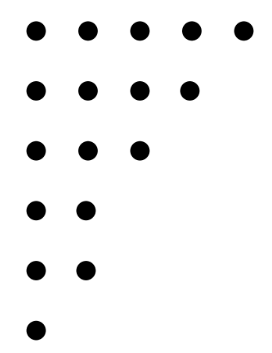
\includegraphics[width=0.2\textwidth]{slike/11-1.png}
    \caption{$17 = 5 + 4 + 3 + 2 + 2 + 1$}
\end{figure}
\begin{itemize}
    \item Dve particije su međusobno \textbf{konjugovane} ukoliko se Ferersov dijagram jedne dobija transponovanjem Ferersovog dijagrama druge.
    \item Particija je \textbf{samokonjugovana} ako je konjugovana sama sa sobom.
\end{itemize}
\newpage
\begin{theorem}
    Važi:
    \begin{enumerate}
        \item Broj particija broja $n$ na najviše $k$ sabiraka jednak je broju particija broja $n+k$ na $k$ sabiraka.
        \item Broj particija broja $n$ na najviše $k$ sabiraka jednak je broju particija broja $n$ na sabirke iz $\mathbb{N}_k$.
        \item Broj particija broja $n$ na parne sabirke jednak je broju particija broja $n$ u kojima se svaki sabirak pojavljuje paran broj puta.
        \item Broj samokonjugovanih particija broja $n$ jednak je broju particija broja $n$ u kojima su sabirci različiti i neparni.
    \end{enumerate}
\end{theorem}
\begin{proof}
    \begin{enumerate}
        \item Jedan način da se ovo dokaže je direktno iz teoreme \ref{10-3}. Drugi način je preko Ferersovih dijagrama. Naime, neka je data 
        particija broja $n + k$ na $k$ sabiraka. To znači da prva kolona Ferersovog dijagrama sadrži tačno $k$ markera. Ako uklonimo tu prvu kolonu, 
        dobijamo dijagram neke particije broja $n$ koji ima najviše $k$ vrsta, pa dobijena particija broja $n$ ima najviše $k$ sabiraka. Dakle, ovo je bijekcija,
        pa tvrđenje direktno sledi.
        \item Ferersov dijagram particije broja $n$ na najviše $k$ sabiraka je konjugovan dijagramu jedne particije broja $n$ na sabirke iz $\mathbb{N}_k$.
        \item Ferersov dijagram particije broja $n$ na $k$ parnih sabiraka ima $k$ vrsta sa parnim brojem markera u svakoj. Dakle, broj markera u $i$-toj vrsti se od broja markera u $i+1$-toj vrsti razlikuje za $2m, \;m\in \mathbb{N}_0$. Ukoliko je broj elemenata u svakoj vrsti jednak, tada će broj kolona svakako biti paran (jer je broj markera u svakoj vrsti paran). Alternativno, ukoliko postoje 2 uzastopne vrste sa različitim brojem elemenata, kako će njihova razlika biti paran broj, ovo će generisati identične kolone, pa dobijamo tvrđenje.
        \item Može se uspostaviti bijekcija između tzv. "kuka" u jednom Ferersovom dijagramu sa sabircima u drugom dijagramu. Naime, posmatrajmo prvu kuku, koju čine prva kolona i prva vrsta. One imaju zajedničku tačku $(1, 1)$, pa je broj markera $k + k - 1 = 2k-1$. Broj elemenata u kukama opada (jer su ugnježdene), pa dobijamo ono što se tražilo. 
    \end{enumerate}
\end{proof}

\newpage
\section{Rekurentne jednačine. Definicija i rešenja. Linearna rekurentna jednačina i
njeno opšte rešenje. }
\begin{definition}
    Za $n \in \mathbb{N}_0, k\in \mathbb{N}, a_i \in \mathbb{R}$, \textbf{rekurentnom jednačinom} nazivamo jednačinu oblika
    \[ a_{n+k} = \phi(n, a_n, a_{n+1}, \ldots, a_{n+k-1}).\]
    \textbf{Rešenje} rekurentne jednačine je bilo koji niz $(a_n)$ čiji članovi zadovoljavaju tu jednačinu. \textbf{Opšte rešenje} zavisi od $k$ konstanti, tj. članova niza. Različita rešenja se dobijaju iz opšteg izborima vrednosti konstanti. Uslove kojima se jednoznačno određuju vrednosti ovih konstanti zovemo \textbf{početnim uslovima}. Jedno rešenje koje je određeno nekim početnim uslovima zovemo \textbf{partukularno rešenje}. Za prozvoljnu vrednost $n$, $n$-ti član niza zovemo \textbf{opšti član}.
\end{definition}
\begin{itemize}
    \item Linearna rekurentna jednačina $k$-tog reda:
    \[
        f_0(n)a_n + f_1(n)a_{n+1} + \dots + f_k(n)a_{n + k} = f(n)
    \]
    \item Linearne rekurentne jednačine mogu imati konstantne ili funkcionalne koeficijente.
    \item Ako je $f(n) = 0$, onda je jednačina homogena.
    \item Ako je $f_k(n) = 1$, onda je jednačina u normalizovanom obliku.
    \item Rešenja $(a_n^{(1)}), \ldots, (a_n^{(r)})$ su zavisna ako se neko od njih može predstaviti kao lin. kombinacija ostalih.
\end{itemize}
\begin{theorem}
    Rešenja $(a_n^{(1)}), \ldots, (a_n^{(r)})$ homogene jednačine su nezavisna akko
    \[ \begin{vmatrix} 
        a_1^{(1)} & a_1^{(2)} & \ldots & a_1^{(r)} \\ 
        a_2^{(1)} & a_2^{(2)} & \ldots & a_2^{(r)} \\ 
        \vdots & \vdots & \ddots &\vdots \\ 
        a_r^{(1)} & a_r^{(2)} & \ldots & a_r^{(r)} 
    \end{vmatrix} \neq 0\]
\end{theorem}
\begin{proof}\
    \begin{itemize}
        \item $\implies$: \\
        Nezavisnost rešenja daje i nezavisnost kolona-vektora matrice, što znači da je determinanta različita od nule.
        \item $\impliedby$: \\
        Ako je determinanta različita od nule, tada je njen rang jednak $r$, pa su njeni kolona-vektori nezavisni, dakle rešenja su nezavisna.
    \end{itemize}
\end{proof}
\begin{theorem}
    Ukoliko su rešenja $(a_n^{(1)}), \ldots, (a_n^{(r)})$ homogene jednačine nezavisna, tada je opšte rešenje određeno sa
    \[ a_n = c_1a_n^{(1)} + c_2a_n^{(2)} + \ldots + c_ka_n^{(k)}, \;\; c_i \in \mathbb{R} \]
\end{theorem}
\begin{itemize}
    \item Opšte rešenje nehomogene linearne rekurentne jednačine je oblika 
    \[
        a_n = h_n + p_n,
    \]
    gde je $h_n$ opšte rešenje odgovarajuće homogene jednačine, a $p_n$ partikularno rešenje date nehomogene jednačine.
\end{itemize}

\newpage
\section{Linearne rekurentne jednačine sa konstantnim koeficijentima}
\begin{itemize}
    \item Linearna rekurentna jednačina $k$-tog reda sa konstantim koeficijentima:
    \[
        f_0a_n + f_1a_{n+1} + \dots + f_ka_{n + k} = f(n)
    \]    
    \item Karakteristična jednačina rekurentne jednačine sa konstantnim koeficijentima je jednačina
    \begin{equation}
        f_kx^k + \dots + f_1x + f_0 = 0
        \label{lrj1}
    \end{equation}
    \item Određivanje \textbf{opšteg rešenja} linearne rek. jednačine sa konst. koeficijentima:
    \begin{enumerate}
        \item Ako su nule $x_1, x_2, \dots, x_n \in \mathbb{C}$ karakteristične jednačine \ref{lrj1} jednostruke,
        onda je to opšte rešenje dato sa
        \[
            a_n = c_1x^n_1 + c_2x^n_2 + \dots + c_kx^n_k
        \]
        \item Ako postoji nula multipliciteta $m$, onda ona daje član 
        \[
            c_ix_i^n + c_{i+1}nx^n_i + \dots + c_{i + m - 1}n^{m - 1}x_i^n
        \]
        u opštem rešenju homogene jednačine.
    \end{enumerate}
    \item Određivanje \textbf{partikularnog rešenja} lin. rek. jednačine sa konst. koeficijentima:
    \begin{itemize}
        \item Ako važi $f(n) = P_d(n)b^n$, gde je $P_d$ polinom stepena $d$ i $b \in \mathbb{R}$, važi sledeće:
        \begin{enumerate}
            \item ako $x = b$ nije nula kar. jednačine \ref{lrj1}, onda se partikularno rešenje traži u obliku
            \[
                p_n = (A_0 + A_1n + \dots + A_dn^d)b^n            
            \]
            \item ako $x = b$ jeste nula multipliciteta $m$, onda se partikularno rešenje traži u obliku
            \[
                p_n = n^m(A_0 + A_1n+\dots + A_dn^d)b^n
            \]
        \end{enumerate}
    \end{itemize}
    \item Mogu se rešavati i pomoću funkcija generatrisa.
    
\end{itemize}

\section{Funkcije generatrise i rešavanje rekurentnih jednačina.}
\begin{theorem}
    Funkcija generatrisa niza $(a_n)$ određenog rekurentnom jednačinom 
    \[ f_0a_n + f_1a_{n+1}+ \ldots + a_{n+k} = 0, \;\; a_0 = c_0, \ldots, a_{k-1}= c_{k-1} \]
    oblika je
    \[ A(x) = \frac{P(x)}{f_0x^k + f_1x^{k-1} + \ldots + 1}, \]
    gde je $P(x)$ polinom stepena strogo manjeg od $k$.
\end{theorem}
\newpage
\section{Particije skupova. Stirlingovi brojevi 2. vrste i Belovi brojevi. }
\begin{definition}
    Particija skupa $\mathbb{N}_n$ na $k$ podskupova je skup njegovih nepraznih disjunktnih podskupova $S_1, S_2, \ldots, S_k$ td.
    \[ \mathbb{N}_n = S_1 \cup S_2 \cup \dots \cup S_k. \]
    Prazan skup ima jednu particiju.
\end{definition}

\begin{definition}
    Stirlingov broj druge vrste, $S(n, k)$, jednak je broju particija skupa od $n$ elemenata na $k$ podskupova.
\end{definition}

\begin{definition}
    Belov broj, $B(n)$, jednak je broju particija skupa od $n$ elemenata, tj.
    \[ B(n) = \sum_{k=0}^{n} S(n, k) \]
\end{definition}

\begin{theorem}
    \[ S(n + 1, k) = S(n, k - 1) + kS(n, k) \]
\end{theorem}
\begin{proof}
    Sve particije skupa $\mathbb{N}_{n+1}$ na $k$ podskupova se mogu dobiti od particije skupa $\mathbb{N}_n$ na $k-1$ i $k$ podskupova. U prvom slučaju, samo dodamo $\{n + 1\}$ kao $k$-ti podskup (ovo je prvi sabirak sa desne strane).U drugom slučaju, bilo kom od $k$ podskupova možemo dodati element $n+1$ (drugi sabirak).
\end{proof}
\begin{itemize}
    \item početni uslovi za Stirlingove brojeve druge vrste: 
    \[ S(n, 1) = S(n, n) = 1 \]
\end{itemize}
\begin{theorem}
    Belovi brojevi su određeni početnim uslovom $B(0) = 1$ i rek. jednačinom
    \[ B(n+1) = \sum_{k= 0}^{n}{{n} \choose k}B(k) \]
\end{theorem}
\section{Fibonačijevi brojevi. Zlatni presek. Opšti član i funkcija generatrisa
Fibonačijevog niza. }

\begin{itemize}
    \item Fibonačijev niz: \[ F_{n+2} = F_{n+1} + F_n, \;\; F_0 = 0, F_1 = 1 \]
    \item Zlatni presek:
    \[ \frac{d + k}{d} = \frac{d}{k}, \]
    $d > k$, delovi duži. Rešavanjem jednačine za $k = 1$ se dobija
    \[ d_{1/2} = \frac{1 \pm \sqrt{5}}{2} \implies d =  \frac{1 + \sqrt{5}}{2} \approx 1.618\]
\end{itemize}
\begin{theorem}
    Opšti član Fibonačijevog niza:
    \[ F_n = \frac{\bigg(\frac{1 + \sqrt{5}}{2}\bigg)^n - \bigg(\frac{1 - \sqrt{5}}{2}\bigg)^n}{\sqrt{5}} \]
\end{theorem}
\begin{proof}
    Rešavanjem rekurentne jednačine.
\end{proof}

\begin{theorem}
    Opšti član Fibonačijevog niza (zaokruživanje na najbliži ceo broj):
    $$ F_n = \left[ \frac{\bigg(\frac{1+\sqrt{5}}{2}\bigg)^n}{\sqrt{5}} \right] $$
\end{theorem}
\begin{proof}
    \[\left| \frac{\left(\frac{1-\sqrt{5}}{2}\right)^n}{\sqrt{5}} \right| < \frac{1}{2}\]
\end{proof}

\begin{theorem}
    Funkcija generatrisa Fibonačijevog niza:
    \[ F(x) = \frac{x}{1-x-x^2} \]
\end{theorem}

\section{Svojstva Fibonačijevih brojeva.}
\begin{theorem}
    Za $n \geq 1$ važi
    \[
        \frac{F_{n+1}}{F_n} = \underbrace{1 + \frac{1}{1+\frac{1}{1+\frac{1}{\frac{\ddots}{1+\frac{1}{1}}}}}}_n
    \]
\end{theorem}
\begin{proof}
    Matematičkom indukcijom. Za $n=1$ dobijamo $1=1$. Pretpostavimo da jednakost važi za $n-1$.
    \[\frac{F_{n+1}}{F_n} = \frac{F_{n-1} + F_n}{F_n} = 1 + \frac{F_{n-1}}{F_n} = 1 + \frac{1}{\frac{F_n}{F_{n-1}}}\]
\end{proof}
\begin{theorem}
    \[
        \lim_{n \to +\infty} \frac{F_{n+1}}{F_n} = \frac{1+ \sqrt{5}}{2}
    \]
\end{theorem}
\begin{proof}
    \[
        1 < \frac{F_{n+1}}{F_n} < 2 \implies \text{ograničen}
    \]
    Takođe, niz konvergira i važi $L = 1 + \frac{1}{L} \implies L = \frac{1 + \sqrt{5}}{2}.$
\end{proof}
\begin{theorem}
    \[
        F_1 + F_2 + \dots + F_n = F_{n+2} - 1
    \]
\end{theorem}
\begin{proof}
    \[F_1 + F_2 + \dots + F_n = (F_3 - F_2) + (F_4 - F_3) + \dots + (F_{n+2} - F_{n+1}) = F_{n+2} -1\]
\end{proof}
\begin{theorem}
    Za $n \geq 1$ važi
    \[
        F_{n+1}F_{n-1} - F_{n}^2 = (-1)^n
    \]
\end{theorem}
\begin{proof}
    Dokaz indukcijom.
\end{proof}

\section{Lukasovi i Katalanovi brojevi.}
\subsection{Lukasovi brojevi}
\begin{definition}
    Lukasovi brojevi:
    \[ L_{n+2} = L_{n+1} + L_n, \;\; L_0 = 2, L_1 = 1 \]
\end{definition}
\begin{theorem}
    Opšti član niza Lukasovih brojeva:
    \[ L_n = \left( \frac{1 + \sqrt{5}}{2} \right)^n + \left( \frac{1 - \sqrt{5}}{2} \right)^n \]
\end{theorem}
\begin{proof}
    Dokaz rešavanjem rekurentne jednačine.
\end{proof}
\begin{theorem}
    Funkcija generatrisa Lukasovog niza:
    \[
        L(x) = \frac{2-x}{1-x-x^2}
    \]
\end{theorem}
\begin{proof}
    Dokaz rešavanjem rekurente jednačine preko funkcija generatrisa.
\end{proof}
\begin{theorem}
    Za Lukasove i Fibonačijeve brojeve ($n \geq 1$) važi
    \[ L_n = F_{n+1} + F_{n-1} \]
\end{theorem}
\begin{proof}
    Dokaz indukcijom.
\end{proof}
\subsection{Katalanovi brojevi}
\begin{definition}
    Katalanov niz:
    \[ C_n = \sum_{i=0}^{n-1}C_i \cdot C_{n-i-1},\;\; C_0 = 1 \]
\end{definition}
\begin{theorem}
    Opšti član Katalanovog niza:
    \[ C_n = \frac{1}{n+1} {{2n} \choose n} \]
\end{theorem}

\newpage
\tableofcontents
\end{document}